\documentclass[]{BasiliskReportMemo}
\usepackage{AVS}
\usepackage{algorithmic}
\usepackage[boxed]{algorithm}


\newcommand{\submiterInstitute}{Autonomous Vehicle Simulation (AVS) Laboratory}

\newcommand{\ModuleName}{ThrusterForces}
\newcommand{\subject}{Algorithms to Map Desired Torque Vector onto a set of Thrusters }
\newcommand{\status}{Ready}
\newcommand{\preparer}{H. Schaub}
\newcommand{\summary}{Include a short summary of what this system engineering report is about.  Should be 300 words or less.     }


\begin{document}


\makeCover


%
%	enter the revision documentation here
%	to add more lines, copy the table entry and the \hline, and paste after the current entry.
%
\pagestyle{empty}
{\renewcommand{\arraystretch}{1.1}
\noindent
\begin{longtable}{|p{0.5in}|p{4.5in}|p{1.14in}|}
\hline
{\bfseries Rev}: & {\bfseries Change Description} & {\bfseries By} \\
\hline
v0.1 & Updated the thruster force evaluation to account for center of mass offsets & H. Schaub \\
v0.2 & Updated the figure and the $[C]$ matrix notation & H. Schaub \\
v0.3 & The thruster mapping logic has changed, and this documentation now reflects what the new algorithm does. & H. Schaub \\
\hline

\end{longtable}
}

\newpage
\setcounter{page}{1}
\pagestyle{fancy}

\tableofcontents
~\\ \hrule ~\\

\begin{figure}[htb]
	\centerline{
	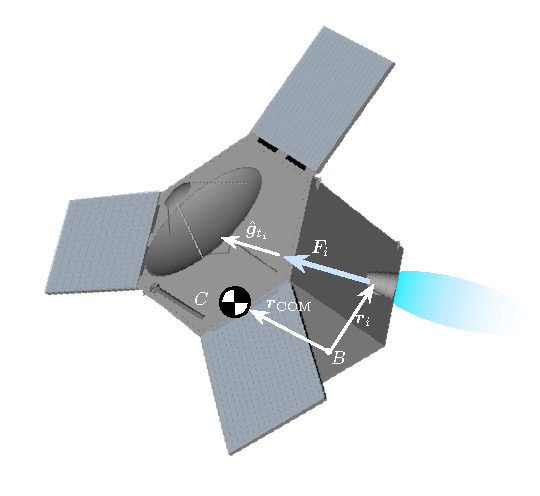
\includegraphics[]{Figures/thrusterNotation}
	}
	\caption{Illustration of the Spacecraft Thruster Notation}
	\label{fig:thruster}
\end{figure}

\section{Introduction}
\subsection{Torque Control Axes}
This technical note describes a general algorithm that maps a desired ADCS external control torque $\bm L_{r}$ onto force commands for a cluster of thrusters.  Let $\hat{\bm c}_{j}$ be the axis about which the thrusters are to produce the desired torque.  The matrix of $N_{c}$ thruster axes rows is then given by
\begin{equation}
	[C]  = \begin{bmatrix}
		\hat{\bm c}_{1} \\ \vdots \\ \hat{\bm c}_{N_{c}}
	\end{bmatrix}
\end{equation}
The module can accept up to 3 orthogonal control axis $\hat{\bm c}_{j}$.  Let $\bar{\bm L}_{r}$ be the three-dimensional reduced set of $\bm L_{r}$ onto the set of control axes, given by:
\begin{equation}
	\bar{\bm L}_{r} = [C]^{T} [C] \bm L_{r}
\end{equation}
The goal of the thruster mapping strategy is to find a set of $\bm F$ thruster forces that yield $\bar{\bm L}_{r}$.  

\subsection{Thruster to Torque Mapping Matrix}
The $i^{\text{th}}$ thruster location relative to the spacecraft point $B$ is given by $\bm r_{i}$ as illustrated in Figure~\ref{fig:thruster}.  The unit direction vector of the thruster force is $\hat{\bm g}_{t_{i}}$, while the thruster force is given by
\begin{equation}
	\label{eq:th:1}
	\bm F_{i} = F_{i} \hat{\bm g}_{t_{i}}
\end{equation}
The toque vector produced by each thruster about the body fixed point $C$ is thus
\begin{equation}
	\bm \tau_{i} = (\bm r_{i} - \bm r_{\text{COM}}) \times F_{i}  \hat{\bm g}_{t_{i}}
\end{equation}
The total torque onto the spacecraft, due to a cluster of $N$ thrusters, is
\begin{equation}
	\tau_{j} = \sum_{i=1}^{N} \bm \tau_{i} 
	= \sum_{i=1}^{N}  ((\bm r_{i} - \bm r_{\text{COM}}) \times \hat{\bm g}_{t_{i}}) F_{i} = \sum_{i=1}^{N}  \bm d_{i} F_{i}
\end{equation}
where 
\begin{equation}
	\label{eq:th1:1}
	\bm d_{i} =    ( \bm r_{i} - \bm r_{\text{COM}})  \times \hat{\bm g}_{t_{i}}
\end{equation}
In matrix form, the net spacecraft torque is written compactly as
\begin{equation}
	\label{eq:DF}
	 \bm\tau = \begin{bmatrix}
		 \bm d_{1} \cdots  \bm d_{N}
	\end{bmatrix} \begin{bmatrix}
		F_{1} \\
		\vdots \\
		F_{N}
	\end{bmatrix} = [D] \bm F
\end{equation}
where $[D]$ is a $3\times N$ matrix that maps the thruster forces $F_{i}$ to the spacecraft torque $\bm \tau$. 


\section{ACS Thruster Force Algorithm for a Thruster Configuration with Full Torque Controllability}
Here a thruster configuration is assumed that can produce pure torque-couples without exerting a net torque onto the spacecraft.  The thrusters force values $F_{i}$ must be strictly non-negative (i.e. either 0 or positive).   Note that in this configuration having all thrusters on will produce zero net force and torque onto the spacecraft.  Thus the $F_{i} = F_{j}$ solution is in the nullspace of the mapping in Eq.~\eqref{eq:DF}.  

The goal of the thruster force algorithm is to determine a set of thruster forces $\bm F$ such that the net force onto the spacecraft is
\begin{equation}
	\label{eq:th:2}
	\bm\tau = \bar{\bm L}_{r}  = [D]\bm F
\end{equation}
without bleeding torque onto the un-controlled axes.  The first step is to perform a standard minimum norm inverse solution using
\begin{equation}
	\label{eq:th:min}
	\bm F = [D]^{T}([D][D]^{T})^{-1} \bar{\bm L}_{r}
\end{equation}
The $3\times 3$ matrix $[D][D]^{T}$ is full rank and thus invertible with the assumption that this RCS configuration has a full 3D torque controllability.  This set of of thruster forces will contain $F_{i}$ values that are both positive and negative.  Next, to achieve strictly non-negative values, the minimum $F_{i}$ value is determined and subtracted from all $N$ force values.  
\begin{equation}
	\bm F \leftarrow \bm F -  \text{min}(\bm F)
\end{equation}
The resulting set of $F_{i}$ forces will produce the desired control torque $\bar{\bm L}_{r}$ and achieve a net zero force onto the spacecraft.  The latter results is due to the assumption off an ACS thruster configuration that can produce pure moment couples.  



\section{2-Stage Minimum Norm ACS Thruster Mapping Algorithm}
To increase the robustness of the sign-constrained minimum norm thruster force solution, as 2nd stage is included if the number of available ACS thrusters is not equal to the number of installed thrusters.  This simulates scenarios where some thrusters are now offline.    The minimum norm solution from the earlier solution is first evaluated, and then shifted by subtracting the minimum $F_{i}$ value.  

Each thruster can only produce a positive force.  With off-pulsing, the nominal thrust force plus the negative correction must still yield a non-negative thrust force.  The module parameter {\tt thrForceSign} is either +1 or -1 to account for the desired force sign.  The value of this parameter is represented through $s_{F}$.  With the ACS thruster configuration this value would always be +1.  

We assume that $\bm F$ elements only contain forces that are either zero or values with the desired sign.   Assume there are $M$  force values in $\bm F$ with a sign that matches $s_{F}$.  The locations of these values is provided in the $N$-dimensional array $\bm t_{\text{used}}$ which contains either 0 or 1 values.  For example, consider $N=8$ and only thrusters 2 and 6 produce  zero forces. In this case we find
\begin{equation}
	\bm t_{\text{used}} = \begin{bmatrix}
		1 & 0 & 1 & 1 & 1 & 0 & 1 & 1
	\end{bmatrix}
\end{equation}
This reduces the thruster force search to a subset of $M$ thrusters.  Let $\bar{\bm F}_{j}$ be a $M\times 1$ matrix of to be determined thruster forces.  The corresponding $3\times M$ mapping matrix $[\bar D]$ that projects $\bar{\bm F}$ onto a net body torque about point $B$ is defined as:
\begin{equation}
	[\bar D] = \begin{bmatrix} \bar{\bm d}_{1} & \cdots & \bar{\bm d}_{M} \end{bmatrix}
\end{equation}
with
\begin{equation}
	\bar{\bm d}_{i} = (\bm r_{i} - \bm r_{\text{COM}}) \times \hat{\bm g}_{i}
\end{equation}
The net torque due to $\bar{\bm F}$ is 
\begin{equation}
	\bar{\bm \tau} = [\bar D] \bar{\bm F}
\end{equation}

A modified set of thruster force solutions $\bar{\bm F}$ to generate the desired torque $\bar{\bm L}_{r}$ is found through a second minimum norm operation:
\begin{equation}
	\label{eq:th:min2}
	\bar{\bm F} = [\bar D]^{T}([\bar D][\bar D]^{T})^{-1} \bar{\bm L}_{r}
\end{equation}




The next step is to sum the individual $\bar{\bm F}$ thruster solutions to the yield the net set of thruster forces required to produce $\bar{\bm L}_{r}$.  This is done using the  $\bm t_{\text{used}}$ matrix to determine which thrusters have non-zero contributions.   The final step is to evaluate the minimum $F_{i}$ force again and subtract this from all thruster force values.




\section{DV Thruster Firing Strategy}
With a DV thruster configuration the thruster force axes are parallel.  As such, this configuration cannot produce a torque along the DV thrust axis.  A slightly modified version of the above algorithm is used in this case.  With the DV configuration the attitude along the axes orthogonal to the thrust vector are controlled via off-pulsing.  As such, the thruster firing mapping must produce negative $F_{i}$ values and the {\tt thrForceSign} sign must be set to -1.  

The modified algorithm still evaluates the first minimum norm inverse, but does not subtract out the $\text{min}(\bm F)$ value.  Rather, the 2nd stage is used to determine which DV thrusters produce the torque with a negative torque value to generate the corresponding $[\bar D]$ matrix.  After performing the 2nd minimum norm inverse with $[\bar D]$ the subtraction of  $\text{min}(\bm F)$ is not performed.  






\section{Performance Illustration}
\subsection{ACS Thruster Configuration}
To illustrate the performance of this algorithm, the following simulation setup is used.  Let the ACS system have a total of $N = 8$ thrusters with the following body-fixed locations:
\begin{gather*}
	\label{eq:th:loc}
	\bm r_{1} = \begin{bmatrix} +1.125, 0.0, +0.75  \end{bmatrix}^{T} \text{ m}
	\quad\quad
	\bm r_{2} = \begin{bmatrix} -1.125, 0.0, +0.75  \end{bmatrix}^{T} \text{ m}
	\\
	\bm r_{3} = \begin{bmatrix} -1.125, 0.0, +0.75  \end{bmatrix}^{T}	 \text{ m}
	\quad\quad
	\bm r_{4} = \begin{bmatrix} +1.125, 0.0, +0.75  \end{bmatrix}^{T} \text{ m}
	\\
	\bm r_{5} = \begin{bmatrix} +1.125, 0.0, -0.75  \end{bmatrix}^{T}	 \text{ m}
	\quad\quad
	\bm r_{6} = \begin{bmatrix} -1.125, 0.0, -0.75  \end{bmatrix}^{T} \text{ m}
	\\
	\bm r_{7} = \begin{bmatrix} -1.125, 0.0, -0.75  \end{bmatrix}^{T}	 \text{ m}
	\quad\quad
	\bm r_{8} = \begin{bmatrix} +1.125, 0.0, -0.75  \end{bmatrix}^{T} \text{ m}
\end{gather*}
with the force unit direction vectors:
\begin{gather*}
	\label{eq:th:gt}
	\bm g_{t_{1}} = \begin{bmatrix} +0.707107, +0.707107, 0  \end{bmatrix}^{T}
	\quad\quad
	\bm g_{t_{2}} = \begin{bmatrix} -0.707107, +0.707107, 0  \end{bmatrix}^{T}
	\\
	\bm g_{t_{3}} = \begin{bmatrix} -0.707107, -0.707107, 0  \end{bmatrix}^{T}
	\quad\quad
	\bm g_{t_{4}} = \begin{bmatrix} +0.707107, -0.707107, 0  \end{bmatrix}^{T}
	\\
	\bm g_{t_{5}} = \begin{bmatrix} +0.707107, +0.707107, 0 \end{bmatrix}^{T}
	\quad\quad
	\bm g_{t_{6}} = \begin{bmatrix} -0.707107, +0.707107, 0  \end{bmatrix}^{T}
	\\
	\bm g_{t_{7}} = \begin{bmatrix} -0.707107, -0.707107, 0  \end{bmatrix}^{T}
	\quad\quad
	\bm g_{t_{8}} = \begin{bmatrix} +0.707107, -0.707107, 0  \end{bmatrix}^{T}
\end{gather*}
\begin{figure}[htb]
	\centerline{
	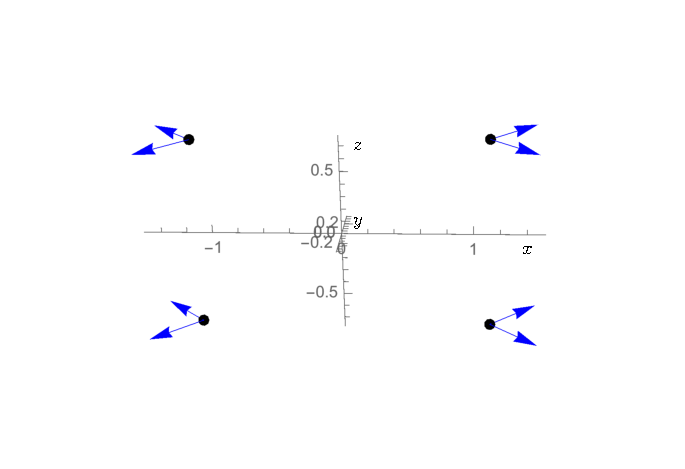
\includegraphics[]{Figures/8ThrConfig}
	}
	\caption{Illustration of an 8-thruster ACS configuration}
	\label{fig:8ThrConfig}
\end{figure}
\begin{figure}[p]
	\centering
	\subfigure[Percent Torque Error]
	{\label{fig:minTorquePer}
	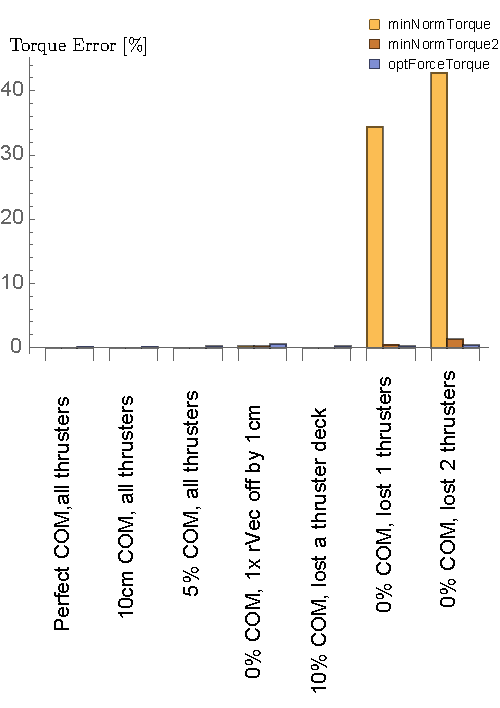
\includegraphics[width=0.45\textwidth]{Figures/minTorquePer}} 
	\\
	\subfigure[Thruster Control Implementation Effort]
	{\label{fig:minTorqueSumF} 
	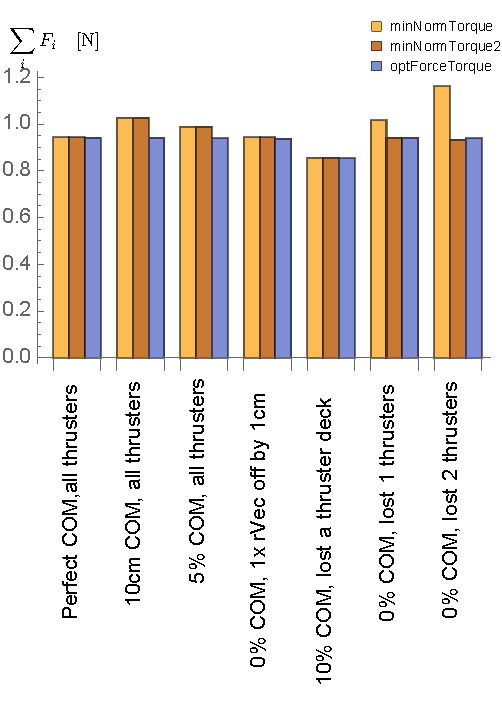
\includegraphics[width=0.45\textwidth]{Figures/minTorqueSumF}}  
	\subfigure[Net Thruster Disturbance Force]
	{\label{fig:minTorqueNetF} 
	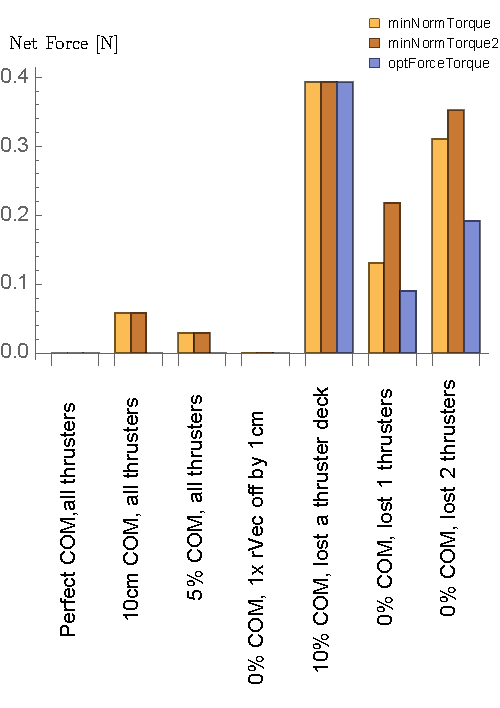
\includegraphics[width=0.45\textwidth]{Figures/minTorqueNetF}}  
	\caption{ACS Thruster Mapping Performance Mapping Illustration Comparing the 1-stage and 2-stage minimum norm solution to the thruster mapping of a nonlinear optimization solution.}
	\label{fig:minTorque}
\end{figure}


The resulting configuration is illustrated in Figure~\ref{fig:8ThrConfig}.  In this setup the center of mass position vector is set to $\bm r_{\text{COM}} = (0,0,0)^{T} \text{ m}$.  The following plots show the thruster firing performance by considering a rang of scenarios.  The first case assumes all thrusters are available, and the $\bm r_{\text{COM}}$ vector is known perfectly.  The second and third case also have all thrusters available, but the $\bm r_{\text{COM}}$ vector knowledge is off by 10cm or 5cm in the $z$ direction.  The 4th case has the perfect $\bm r_{\text{COM}}$ vector, but the first thruster location is off by 1cm in the $y$ direction.  The 5th case again assumes a 10cm COM offset, but also that only 4/8 thrusters are available.  In essence, all the lower or upper thruster have become un-available.  The 6th and 7th case assumes perfect COM knowledge, but either the last one or last two thrusters are un-available.  


The resulting performance is illustrated in Figure~\ref{fig:minTorque}.  Here 20 random $\bm L_{r}$ torques are generated, and the mean results are shown.  The $[C]$ matrix is set to the identity matrix to control all three axes.   The 1-stage minimum norm algorithm is compared to an optimal thruster firing solution which minimizes the net thruster forces used, the net disturbance torque onto the craft, all subject to producing the desired control torque.    Regarding generating the desired control torque, only when 1 or 2 thrusters were lost did the algorithm have issues generating the required torque.  In all other cases the desired torque was always produced as shown in Figure~\ref{fig:minTorquePer}.  In comparison, the 2-stage minimum norm algorithm performs very well in these latter cases where 1-2 thrusters are lost, yielding only very small torque errors on average.  

The control effort required to achieve this torque is shown in Figure~\ref{fig:minTorqueSumF}.  Here the $F_{i}$ thruster force values are simply summed to have a sense of how much on-time or fuel is required for a given scenario.  If all ACS thrusters are operating and the COM is perfectly modeled is the control effort equivalent to the optimal solution.  In all other case the effort is about 10-20\% larger.  in contrast, the 2-stage minimum norm algorithm control efforts in the cases with lost thrusters is very similar to those of the optimal answers.  This illustrates the robustness achieved by adding this 2nd stage if some thrusters are lost.  

Finally, to see how well this algorithm is able to avoid net disturbance forces onto the spacecraft, the results in Figure~\ref{fig:minTorqueNetF} are shown.  Overall the 1-stage algorithm did well, producing 0 net force in the ideal case and the case where the 1st thruster location is different, and matches the optimal answer for the lost thruster deck and lost single thruster case.  In the other cases there is some net disturbance force.  The 2-stage algorithm only differs here when thrusters are lost.  Here the net disturbance torque is higher than the 1-stage solution.  However, this is an expected result as the 1-stage solution produces huge torque errors, while the 2-stage solution produces a very different thruster solution which yields very small torque errors. 

Overall the 2-stage thruster firing performs very well in comparison to the the optimal thruster firing solutions.  The optimal solutions are computationally very expensive and not suitable to realtime flight-software implementations.  








\subsection{DV Thruster Configuration}
Next consider a DV thruster configuration where the off-thruster-axis control torques are produces through off-pulsing.  Let the DV system have a total of $N = 6$ thrusters with the following body-fixed locations:
\begin{align*}
	\label{eq:th:loc}
	\bm r_{1} &= \begin{bmatrix} 0, 0.413, -0.1671  \end{bmatrix}^{T} \text{ m}
	& 
	\bm r_{2} &= \begin{bmatrix} 0.357668, 0.2065, -0.1671  \end{bmatrix}^{T} \text{ m}
	\\
	\bm r_{3} &= \begin{bmatrix} 0.357668, -0.2065, -0.1671 \end{bmatrix}^{T}	 \text{ m}
	&
	\bm r_{4} &= \begin{bmatrix} 0, -0.413, -0.1671  \end{bmatrix}^{T} \text{ m}
	\\
	\bm r_{5} &= \begin{bmatrix} -0.357668, -0.2065, -0.1671  \end{bmatrix}^{T}	 \text{ m}
	&
	\bm r_{6} &= \begin{bmatrix} -0.357668, 0.2065, -0.1671 \end{bmatrix}^{T} \text{ m}
\end{align*}
with the force unit direction vectors given by $\hat{\bm g}_{t_{i}} = (0,0,1)^{T}$ as illustrated in Figure~\ref{fig:6ThrConfig}.
\begin{figure}[t]
	\centerline{
	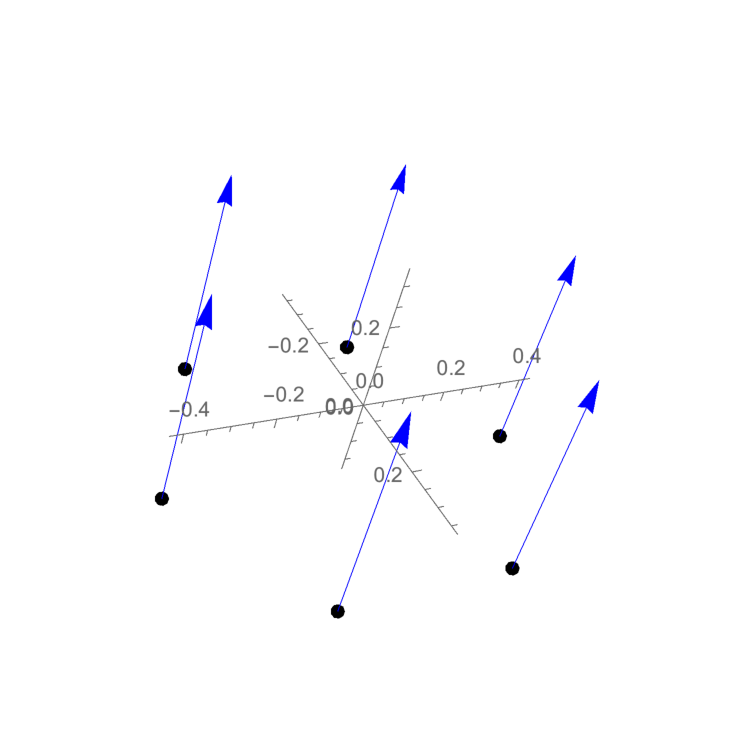
\includegraphics[width=0.4\textwidth]{Figures/dvThrConfig}
	}
	\caption{Illustration of an 6-thruster DV configuration}
	\label{fig:6ThrConfig}
\end{figure}


\begin{figure}[t]
	\centering
	\subfigure[Percent Torque Error]
	{\label{fig:minTorquePerDV}
	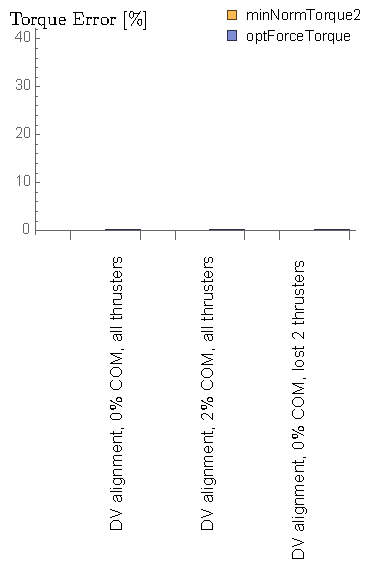
\includegraphics[width=0.4\textwidth]{Figures/dvTorquePer}} 
	\subfigure[Thruster Control Implementation Effort]
	{\label{fig:minTorqueSumFDV} 
	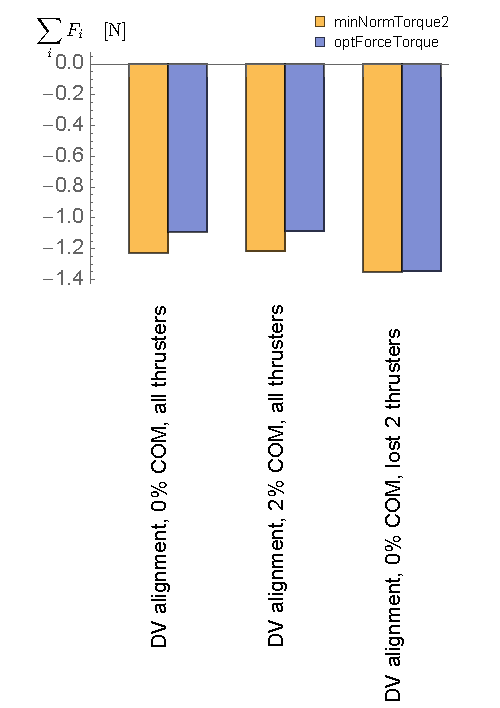
\includegraphics[width=0.45\textwidth]{Figures/dvSumF}}  
	\caption{DV Thruster Mapping Performance Mapping Illustration Comparing the 1-stage and 2-stage minimum norm solution to the thruster mapping of a nonlinear optimization solution.}
	\label{fig:minTorqueDV}
\end{figure}

Figure~\ref{fig:minTorqueDV} illustrates the DV off-pulsing performance for 3 scenarios.  The 1st one has all thrusters available and no COM error.  The 2nd case adds 2cm COM offsets to the $x$ and $y$ axes, while the 3rd case has no COM error but lost an opposing set of thrusters.  Again 20 random $\bm L_{r}$ vectors are generated and the mean performance evaluated.  As only torques about the $x$ and $y$ axis can be controlled with this DV thruster configuration, the control axis matrix is set to 
$$
	[C] = \begin{bmatrix}
		1 & 0 & 0 \\
		0 & 1 & 0
	\end{bmatrix}
$$

The torque implementation errors are compared in Figure~\ref{fig:minTorquePerDV}.  The 2-stage process outlined above is able to produce the required torques in all cases, illustrating good robustness to COM offsets and loosing 2/6 thrusters.  Figure~\ref{fig:minTorqueSumFDV} illustrates the net off-pulsing effort required to achieve these random control torque vectors.  The 2-stage algorithms requires slightly more off-pulsing than the optimal solution.  However, the difference isn't very large, especially in comparison to the drastically faster computational evaluation time.  





















\section{Module Parameters}
\subsection{$\epsilon$ Parameter}
The minimum norm inverse requires a non-zero determinant value of $[D][D]^{T}$.  For this setup, this matrix is a scalar value
\begin{equation}
	D_{2} = \text{det}([D][D]^{T})
\end{equation}
If this $D_{2}$ value is near zero, then the full 3D $\bar{\bm L}_{r}$ vector cannot be achieved.  A common example of such a scenario is with the DV thruster configuration where all $\hat{\bm g}_{t_{i}}$ axes are collinear.  Torques about these thrust axes cannot be produced.  In this case, the minimum norm solution is adjusted to only match the torques along the control matrix $[C]$ sub-space.  Torques being applied outside of $\hat{\bm c}_{j}$ is not possible as $D_{2}$ is essentially zero, indicating the other control axis cannot be controlled with this thruster configuration.  

The minimum norm torque solution is now modified to use
\begin{equation}
	\bar{\bm F} = ([C][\bar D])^{T}( [C][\bar D][\bar D]^{T}[C]^{T})^{-1} [C] {\bm L}_{r}
\end{equation}
As the thruster configuration cannot produce a general 3D torque, here the $[C]$ matrix must have either 1 or 2 control axes that are achievable with the given thruster configuration.  

To set this epsilon parameter, not the definition of the $[D]$ matrix components $\bm d_{i} = (\bm r_{i} \times \hat{\bm g}_{t_{i}})$. Note that $\bm r_{i} \times \hat{\bm g}_{t_{i}}$ is a scaled axis along which the $i^{\text{th}}$ thruster can produce a torque.  The value $\bm d_{i}$ will be near zero if the dot product of this axis with the current control axis $\hat{\bm c}_{j}$ is small.  

To determine an appropriate $\epsilon$ value, let $\alpha$ be the minimum desired angle to avoid the control axis $\hat{\bm c}_{j}$ and the scaled thruster torque axis $\bm r_{i} \times \hat{\bm g}_{t_{i}}$ being orthogonal.  If $\bar r$ is a mean distance of the thrusters to the spacecraft center of mass, then the $d_{i}$ values must satisfy
\begin{equation}
	\frac{d_{i}}{\bar r} > \cos(90\dg - \alpha) = \sin\alpha
\end{equation}
Thus, to estimate a good value of $\epsilon$, the following formula can be used
\begin{equation}
	\epsilon \approx d_{i}^{2} = \sin^{2}\!\alpha \ \bar{r}^{2}
\end{equation}
For example, if $\bar{r} = 1.3$ meters, and we want $\alpha$ to be at least 1$\dg$, then we would set $\epsilon = 0.000515$.

\subsection{$[C]$ matrix}
The module requires control control axis matrix $[C]$ to be defined.  Up to 3 orthogonal control axes can be selected.  Let $N_{c}$ be the number of control axes.  The $N_{c}\times 3$ $[C]$ matrix is then defined as
\begin{equation}
	[C] = \begin{bmatrix}
		\hat{\bm c}_{1}
		\\
		\vdots
	\end{bmatrix}
\end{equation}

Not that in python the matrix is given in a 1D form by defining {\tt controlAxes\_B}.  Thus, the $\hat{\bm c}_{j}$ axes are concatenated to produce the input matrix $[C]$. 

\subsection{{\tt thrForceSign} Parameter}
Before this module can be run, the parameter {\tt thrForceSign} must be set to either +1 (on-pulsing with the ACS configuration) or -1 (off-pulsing with the DV configuration).


\bibliographystyle{unsrt}
\bibliography{references}



\end{document}
